\documentclass[../Maxima_Workbook.tex]{subfiles}

\begin{document}
	
\chapter{Differential Equations}

\section{Introduction}

\subsection{Overview}

Only a small portion of the ODEs encounterd in research and engineering have known exact solutions and can be solved by analytical methods. Even if they can, sometimes their solutions involve complicated expressions with special functions and are of no real help. In this case, the user might prefer to look for an approximate numerical solution instead.

\lz Maxima cannot solve PDEs.

\subsubsection{Analytical methods}

\lz Maxima provides function \hyl{ode2}{\emph{ode2}} to analytically find the general solution of elementary (not necessarily linear) ODEs of first or second order. On the basis of this solution, the initial value problem can be solved by \hyl{ic1}{\emph{ic1}} or \hyl{ic2}{\emph{ic2}}, depending on the order of the ODE. Function \hyl{bc2}{\emph{bc2}} solves the boundary value problem.

\lz In addition, David Billinghurst has developed a new package \emph{contrib\_ode} which employs some more methods for solving first order ODEs and linear homogeneous second order ODEs.

\lz A linear ODE of order n or a system of such ODEs can be solved by \hyl{desolve}{\emph{desolve}} which uses Laplace transformation.

\lz Maxima cannot solve nonlinear ODEs of higher order by analytical means. Note that any (system of) higher order ODE(s) can be transformed into a system of first order ODEs. If this resulting system is linear, it can possibly be solved with \emph{desolve}.

\subsubsection{Numerical methods}

\subsubsection{Graphical methods}

\section{Analytical solution}

\subsection{Ordinary differential equation (ODE) of  1. or 2. order}

\subsubsection{Find general solution}

\paragraph{ode2} \mbox{}\label{DE3}

\lzz \hyt{ode2}{\tcr{\emph{ode2 (eq, depvar(indepvar), indepvar)}}} \hfill \tcr{[function]}\index{ode2}

\lz Solves an ordinary differential equation (ODE) of first or second order. \emph{ode2} takes three arguments: the ODE (not necessarily in explicit form) given by \emph{eq}, the dependent variable \emph{depvar}, and the independent variable \emph{indepvar}. Note that indepvar has to be specified as the argument of depvar again. When successful, \emph{ode2} returns either an explicit or implicit solution for the dependent variable. \emph{\%c} is used to represent the integration constant in the case of first-order equations, \emph{\%k1} and \emph{\%k2} are the constants for second-order equations. 

\lz Derivatives have to be specified in \emph{eq} without quoting function \emph{diff}. The dependence of the dependent variable and its derivative(s) on the independent variable always has to be indicated in \emph{eq}, as in the case of function \emph{desolve}. E.g. in \emph{eq} the dependent variable is written as \emph{y(x)} and not as \emph{y}, and its derivative is written as \emph{diff(y(x),x)} and not as \emph{diff(y,x)}. 

\lz If ode2 cannot obtain a solution for whatever reason, it returns \emph{false}, after perhaps printing out an error message. 

\lz The methods implemented for \emph{first order ODEs}, in the order in which they are tested, are: linear, separable, exact (perhaps requiring an integrating factor), homogeneous, Bernoulli’s equation, and a generalized homogeneous method. 

\lz The types of \emph{second-order ODEs} which can be solved are: constant coefficients, exact, linear homogeneous with non-constant coefficients which can be transformed to constant coefficients, the Euler or equi-dimensional equation, equations solvable by the method of variation of parameters, and equations which are free of either the independent or of the dependent variable so that they can be reduced to two first order linear equations to be solved sequentially.

\lz In the course of solving ODE’s, several variables are set purely for informational purposes: \emph{method} denotes the method of solution used (e.g., linear), \emph{intfactor} denotes any integrating factor used, \emph{odeindex} denotes the index for Bernoulli’s method or for the generalized homogeneous method, and \emph{yp} denotes the particular solution for the variation of parameters technique.

\lz Note that Maxima does not take into consideration the domain of the independent variable, or whether it is simply connected. Neither does Maxima return the precise domain of a solution or any singularities. All his has to be worked out manually, if necessary.

\lz As an example, we wish to solve the following ODE describing a free harmonic oscillator without damp, Satz \ref{P-G43}, given by
\begin{equation}\label{DE4}
	\frac{d^2\vap}{dt^2} + \frac{g}{l} \vap(t)=0
\end{equation}
under the assumptions that $ g, l >0 $. We will continue this example for an IWP to be solved by \emph{ic2}, and later we will solve equation and IWP again with the help of \emph{desolve} to show the differences.

\lz \begin{small}
\color{blue} \leqn
\begin{lstlisting}
<@\tcr{(\%i1)}@   assume(g>0,l>0)$
<@\tcr{(\%i2)}@   eq:diff(<@$\vap$@(t),t,2)+g/l*<@$\vap$@(t);
\end{lstlisting}
\vspace{-5mm} \[\tag*{\tcr{\ttfamily (\%o2)}} \frac{{{d}^{2}}}{d {{t}^{2}}} \vap(t) +\frac{g}{l} \vap(t) \]
\vspace{-6mm} \begin{lstlisting}
<@\tcr{(\%i3)}@   gensol: ode2(eq,<@$\vap$@(t),t),rootscontract;
\end{lstlisting}
\vspace{-5mm} \[\tag*{\tcr{\ttfamily (\%o3)}} \vap(t) =\mathit{\% k1} \sin{\left( \sqrt{\frac{g}{l}} t\right) }+\mathit{\% k2} \cos{\left( \sqrt{\frac{g}{l}} t\right) } \]
\color{black} \reqn
\end{small}
\vspace{-2mm} 

Note that one side of the equation can be omitted, because it is zero, see sect. \ref{Ex1}. Note also that the solution returned by ode2 is not an assignment, it does not bind the variable $ \vap $. The constants \emph{\%k1}, \emph{\%k2} inserted by Maxima can be specified by solving an initial value problem, see function \emph{ic2}, or a boundary value problem, see function \emph{bc2}.

\paragraph{\texorpdfstring{contrib\_ode}{contrib_ode}} \mbox{}

\lzz \hyt{contrib\_ode}{\tcr{\emph{contrib\_ode (eq, depvar, indepvar)}}} \hfill \tcr{[function of contrib\_ode]}\index{ode}

\lz This function makes uses of more methods than \emph{ode2} for solving linear and non-linear first order ODEs as well as linear homogeneous second order ODEs.

\lz load('contrib\_ode)

\subsubsection{Solve initial value problem (IVP)}

\paragraph{1. order ODE: ic1} \mbox{}

\lzz \hyt{ic1}{\tcr{\emph{ic1 (gensol, $ x=x_0, \, y=y_0 $)}}} \hfill \tcr{[function]}\index{ic1}

\lz Solves an initial value problem (IVP) for a first order ordinary differential equation. The first argument \emph{gensol} is a general solution of the ODE as returned by \emph{ode2}. The second argument specified the name and initial value of the independent variable.\footnotemark The last argument gives the name and the initial value of the dependent variable, where $ y_0=y(x_0) $. 

\paragraph{2. order ODE: ic2}\label{DE1} \mbox{}

\lzz \hyt{ic2}{\tcr{\emph{ic2 (gensol, $ x=x_0, \, y=y_0, \, 'diff(y,x)=y_1 $)}}} \hfill \tcr{[function]}\index{ic2}

\lz Solves an initial value problem for a second order ordinary differential equation. The first argument \emph{gensol} is a general solution of the ODE as found by \emph{ode2}. The second argument specifies the name and initial value of the independent variable.\addtocounter{footnote}{-1}\footnotemark \footnotetext{The value of $ x_0 $ does not have to be zero. Any point in the domain of y can be selected.} Then follows the name and the initial value of the dependent variable, where $ y_0=y(x_0) $. The last argument gives the initial value of the first derivative of the dependent variable with respect to the independent variable, evaluated at $ x_0 $.\footnote{Although quoting diff is not absolutely necessary, it is recommended, because sometimes this will prevent unexpected errors from occurring.}

\lz As an example, we want to solve the IVP for the general solution of the oscillator equation found in the example to function \emph{ode2}, first with initial values $ t=0, \; \vap(t)=1, \; \vap(t)'=0 $, then with $ t=0, \; \vap(t)=1, \; \vap(t)'=1 $.

\lz \begin{small}
\color{blue} \leqn
\begin{lstlisting}
<@\tcr{(\%i4)}@   ivpsol: ic2(gensol,t=0,<@$\vap$@=1,'diff(<@$\vap$@,t)=0),rootscontract;
\end{lstlisting}
\vspace{-4mm} \[\tag*{\tcr{\ttfamily (\%o4)}} \vap =\cos{\left( \sqrt{\frac{g}{l}} t\right) } \]
\vspace{-4mm} \begin{lstlisting}
<@\tcr{(\%i5)}@   ivpsol: ic2(gensol,t=0,<@$\vap$@=1,'diff(<@$\vap$@,t)=1),rootscontract;
\end{lstlisting}
\vspace{-4mm} \[\tag*{\tcr{\ttfamily (\%o5)}} \vap =\sqrt{\frac{l}{g}} \sin{\left( \sqrt{\frac{g}{l}} t\right) }+\cos{\left( \sqrt{\frac{g}{l}} t\right) } \]
\color{black} \reqn
\end{small} \vspace{-4mm}

\lz As with any result obtained for a differential equation, it should be checked to see whether it is really a solution. We show this for the second case. First we proof that it satisfies the conditions given to \emph{ic2}. In order to avoid error messages, we use \emph{at} rather than \emph{ev} for the derivative.

\lz \begin{small}
\color{blue}
\begin{lstlisting}
<@\tcr{(\%i6)}@   ivpsol,t=0;
<@\tcr{(\%o6)}@			       <@$\vap$@=1
<@\tcr{(\%i7)}@   at(diff(rhs(ivpsol),t),t=0),ratsimp;
<@\tcr{(\%o7)}@			        1
\end{lstlisting}
\color{black}
\end{small} \vspace{-1mm}

\lz Then we insert the result in our equation \emph{eq}. The following input is equivalent to \hyl{ev}{\emph{ev}}(eq, ivpsol, diff, ratsimp) and causes \emph{rhs(ivpsol)} to be substituted for $ \vap $ in \emph{eq}, then the differentiations to be carried out and finally a simplification. Note that \hyl{diff-flag}{\emph{diff}} here is not the function but an evaluation flag.

\lz \begin{small}
\color{blue}
\begin{lstlisting}
<@\tcr{(\%i8)}@   eq,ivpsol,diff,ratsimp;
<@\tcr{(\%o8)}@			        0
\end{lstlisting}
\color{black}
\end{small} \vspace{-1mm}

\lz The result is the missing \emph{rhs} of \emph{eq}. Therefore, \emph{ivpsol} is a valid solution of \emph{eq}. Since the solution of the IVP is unique, it is the only solution.

\lz Finally we want to solve the IVP at points other than zero. This time, first we select $ t=\pi/(2*sqrt(g/l)), \; \vap(t)=1, \; \vap(t)'=0 $, then $ t=\pi/(3*sqrt(g/l)), \; \vap(t)=1, \; \vap(t)'=0 $. We see that this works just as well.

\lz \begin{small}
\color{blue} \leqn
\begin{lstlisting}
<@\tcr{(\%i9)}@   ic2(gensol,t=<@$\pi$@/(2*sqrt(g/l)),<@$\vap$@=1,'diff(<@$\vap$@,t)=0),rootscontract;
\end{lstlisting}
\vspace{-4mm} \[\tag*{\tcr{\ttfamily (\%o9)}} \vap =\sin{\left( \sqrt{\frac{g}{l}} t\right) } \]
\vspace{-5mm} \begin{lstlisting}
<@\tcr{(\%i10)}@  ic2(gensol,t=<@$\pi$@/(3*sqrt(g/l)),<@$\vap$@=1,'diff(<@$\vap$@,t)=0)$
<@\tcr{(\%i11)}@  PullFactorOut([%,2,1],sqrt(3)/2)$
<@\tcr{(\%i12)}@  PullFactorOut([%,2,2],1/2),rootscontract;
\end{lstlisting}
\vspace{-4mm} \[\tag*{\tcr{\ttfamily (\%o12)}} \vap =\left( \tcr{\frac{\sqrt{3}}{2}}\right)  \sin{\left( \sqrt{\frac{g}{l}} t\right) }+\left( \tcr{\frac{1}{2}}\right)  \cos{\left( \sqrt{\frac{g}{l}} t\right) } \]
\color{black} \reqn
\end{small} \vspace{-4mm}

\lz The result can be checked in the same way as we demonstrated above.

\lz In sect. \ref{DE2} we will demonstrate this same example using function \hyl{desolve}{\emph{desolve}}, and in sect. \ref{IT1} we redo it with \hyl{laplace}{\emph{laplace}}. 

\lz We see that the oscillation function $ \vap $ returned can be a cos or a sin, but generally is a combination of both, with an angular frequency being identical for the sin and the cos, and factors depending on the specific IVP. In sect. \ref{RP2} we will continue this example using pattern matching to transform the oscillation function as returned by \emph{ic2} into the form
\begin{equation*}
	\vap = A \sin (\om t + \alpha)
\end{equation*}
with the amplitude A, the angular frequency $ \om $ and the phase shift $ \alpha $.

\subsubsection{Solve boundary value problem (BVP): bc2}

For a first order ODE, the boundary value problem (BVP) is equivalent to the initial value problem.

\lzz \hyt{bc2}{\tcr{\emph{bc2 (gensol, ival1, depval1, ival2, depval2)}}} \hfill \tcr{[function]}\index{bc2}

\lz Solves a boundary value problem for a second order differential equation. The first argument \emph{gensol} is a general solution to the equation as found by \emph{ode2}; \emph{ival1} specifies the value of the independent variable in a first point, in the form $ x = x_1 $, and \emph{depval1} gives the value of the dependent variable in that point, in the form $ y = y_1 $. The expressions \emph{ival2} and \emph{depval2} give the values for these variables at a second point, using the same form.

\subsection{System of linear ODEs: desolve}\label{DE2}

\lz \hyt{desolve}{\tcr{\emph{desolve (eq, $ y(x) $) $ \gbar $}}} \hfill \tcr{[function]}\index{desolve}

\tcr{\emph{desolve ([$ eq_1,\dots,eq_m $],[$ y_1(x),\dots,y_m(x) $])}}

\lz Solves one or a system of linear ordinary differential equations of order n using Laplace transform. The first argument gives one or a list of differential equations being in the dependent variables y or $ y_1,\dots,y_m $, each of them depending on the independent variable x. Derivatives are given in the equation by quoting function \emph{diff}. The independent variable is not given explicitely as a third argument, as in the case of function \emph{ode2}, but instead, the functional dependence of the dependent variable(s) and its derivative(s) on the independent variable must be indicated both in the equations and in \emph{desolve}'s second argument. E.g. the dependent variable is written as \emph{y(x)} and not as \emph{y}, and its derivative is written as \emph{'diff(y(x),x)} and not as \emph{'diff(y,x)}. If \emph{desolve} cannot obtain a solution, it returns \emph{false}.


\lz \emph{desolve} returns a general solution specifying integration constants in terms of symbolic initial values of the dependent variables and their derivatives at t=0, with t being the independent variable. If an initial or boundary value problem is to be solved, these values can be defined with \emph{atvalue} prior to calling \emph{desolve}. Note that because \emph{desolve} uses Laplace transform, this is only possible for initial or boundary conditions specified at t=0, with t being the independent variable. If one has initial or boundary conditions imposed elsewhere, one can impose these on the \emph{general} solution returned by \emph{desolve} and eliminate the constants by solving the general solution for them and substituting their values back. Let's demonstrate all this with the same example we used for \emph{ode2} and \emph{ic2}. First we use initial values $ t=0, \; \vap(t)=1, \; \vap(t)'=1 $.

\lz \begin{small}
\color{blue} \leqn
\begin{lstlisting}
<@\tcr{(\%i1)}@   assume(g>0,l>0)$
<@\tcr{(\%i2)}@   eq: 'diff(<@$\vap$@(t),t,2)+g/l*<@$\vap$@(t);
\end{lstlisting}
\vspace{-4mm} \[\tag*{\tcr{\ttfamily (\%o2)}} \frac{{{d}^{2}}}{d {{t}^{2}}} \operatorname{\vap }(t)+\frac{g \operatorname{\vap }(t)}{l} \]
\vspace{-5mm} \begin{lstlisting}
<@\tcr{(\%i3)}@   gensol: desolve(eq,<@$\vap$@(t)),expand,rootscontract;
\end{lstlisting}
\vspace{-4mm} \[\tag*{\tcr{\ttfamily (\%o3)}} \operatorname{\vap }(t)=\sqrt{\frac{l}{g}} \sin{\left( \sqrt{\frac{g}{l}} t\right) } \left( \left. \frac{d}{d t} \operatorname{\vap }(t)\right|_{t=0}\right) +\operatorname{\vap }(0) \cos{\left( \sqrt{\frac{g}{l}} t\right) } \]
\vspace{-5mm} \begin{lstlisting}
<@\tcr{(\%i4)}@   atvalue(<@$\vap$@(t),t=0<@$\footnotemark$@,1)$  atvalue('diff(<@$\vap$@(t),t),t=0<@$\addtocounter{footnote}{-1} \footnotemark$@,1)$
<@\tcr{(\%i5)}@   desolve(eq,<@$\vap$@(t)),expand,rootscontract;
\end{lstlisting}
\vspace{-4mm} \[\tag*{\tcr{\ttfamily (\%o5)}} \operatorname{\vap }(t)=\sqrt{\frac{l}{g}} \sin{\left( \sqrt{\frac{g}{l}} t\right) }+\cos{\left( \sqrt{\frac{g}{l}} t\right) } \]
\color{black} \reqn
\end{small} \vspace{-4mm}
\footnotetext{The value of t here has to be zero, because \emph{desolve} uses Laplace transform.}

\lz The result can be checked in the same way as it was demonstrated for \hyl{ic2}{\emph{ic2}}.

\lz Now we will show how an IVP with initial values at a point other than zero can be solved, selecting $ t=\pi/(3*sqrt(g/l)), \; \vap(t)=1, \; \vap(t)'=0 $, like in the example of \emph{ic2}. Suppose that in the above example we have come untill \begin{small}\tcr{(\%o3)}\end{small}, which is the general solution, but with two unknown variables $ \vap(0) $ and $ \vap'(0) $. We proceed as follows: First we specify our atvalues $ \vap(t) $ and $ \vap'(t) $. With the first of them we go into gensol, evaluated at t. Then we differentiate gensol and go into the result, evaluated at t again, with $ \vap'(t) $. This provides us two equations for the two unknown variables, which we can now solve and substitute back into the general solution. For this last step we use \emph{subst}; \emph{at} doesn't work properly in this case, since one of the variables is itself a noun \emph{at} form. Note also, that we can't use \emph{ev} instead of \emph{at} for the evaluations of \emph{gensol} and \emph{dgensol} at t, also due to the noun \emph{at} form. In an expression like \emph{gensol, t=$ \pi $/(3*sqrt(g/l));} the rhs of the equation would be substituted for t everywhere in \emph{gensol}, including in the noun \emph{at} form. This destroys it and makes it evaluate to zero, giving an incorrect overall result. Here we see that the three seemingly equivalent methods of evaluation at a point (ev, at, subst) have subtle differences that want to be considered carefully. 

\lz \begin{small}
\color{blue} \leqn
\begin{lstlisting}
<@\tcr{(\%i4)}@   atvalue(<@$\vap$@(t),t=t=<@$\pi$@/(3*sqrt(g/l)),1)$
<@\tcr{(\%i5)}@   atvalue('diff(<@$\vap$@(t),t),t=t=<@$\pi$@/(3*sqrt(g/l)),0)$
<@\tcr{(\%i6)}@   at(gensol,t=<@$\pi$@/(3*sqrt(g/l))),ratsimp$  expand(%)$
<@\tcr{(\%i7)}@   PullFactorOut([%,2,1],sqrt(3)/2*sqrt(l/g))$
<@\tcr{(\%i8)}@   at1sol: PullFactorOut([%,2,2],1/2);
\end{lstlisting}
\vspace{-4mm} \[\tag*{\tcr{\ttfamily (\%o8)}} 1=\left( \tcr{\frac{\sqrt{3}\, \sqrt{l}}{2 \sqrt{g}}} \right) \, \left( \left. \frac{d}{d t} \operatorname{\vap }(t)\right|_{t=0}\right) +\operatorname{\vap }(0) \left( \tcr{\frac{1}{2}} \right) \]
\vspace{-5mm} \begin{lstlisting}
<@\tcr{(\%i9)}@   dgensol:diff(gensol,t);
\end{lstlisting}
\vspace{-4mm} \[\tag*{\tcr{\ttfamily (\%o9)}} \frac{d}{d t} \operatorname{\vap }(t)=\sqrt{\frac{g}{l}}\, \sqrt{\frac{l}{g}} \cos{\left( \sqrt{\frac{g}{l}} t\right) } \left( \left. \frac{d}{d t} \operatorname{\vap }(t)\right|_{t=0}\right) -\operatorname{\vap }(0) \sqrt{\frac{g}{l}} \sin{\left( \sqrt{\frac{g}{l}} t\right) } \]
\vspace{-5mm} \begin{lstlisting}
<@\tcr{(\%i10)}@  at(dgensol,t=<@$\pi$@/(3*sqrt(g/l))),ratsimp$
<@\tcr{(\%i11)}@  at2sol:2*sqrt(l)*%;
\end{lstlisting}
\vspace{-4mm} \[\tag*{\tcr{\ttfamily (\%o11)}} 0=\sqrt{l}\, \left( \left. \frac{d}{d t} \operatorname{\vap }(t)\right|_{t=0}\right) -\sqrt{3} \operatorname{\vap }(0) \sqrt{g} \]
\vspace{-5mm} \begin{lstlisting}
<@\tcr{(\%i12)}@  linsolve([rembox(at1sol),at2sol],[<@$\vap$@(0),at('diff(<@$\vap$@(t),t,1),t=0)]);
\end{lstlisting}
\vspace{-4mm} \[\tag*{\tcr{\ttfamily (\%o12)}} [\operatorname{\vap }(0)=\frac{1}{2},\left. \frac{d}{d t} \operatorname{\vap }(t)\right|_{t=0}=\frac{\sqrt{3}\, \sqrt{g}}{2 \sqrt{l}}] \]
\vspace{-5mm} \begin{lstlisting}
<@\tcr{(\%i13)}@ subst((sqrt(3)*sqrt(g))/(2*sqrt(l)),at('diff(<@$\vap$@(t),t,1),t=0),gensol)$
<@\tcr{(\%i14)}@  subst(1/2,<@$\vap$@(0),%),ratsimp$  expand(%)$
<@\tcr{(\%i15)}@  PullFactorOut([%,2,1],sqrt(3)/2)$
<@\tcr{(\%i16)}@  PullFactorOut([%,2,2],1/2),rootscontract;
\end{lstlisting}
\vspace{-4mm} \[\tag*{\tcr{\ttfamily (\%o16)}} \vap(t) =\left( \tcr{\frac{\sqrt{3}}{2}}\right)  \sin{\left( \sqrt{\frac{g}{l}} t\right) }+\left( \tcr{\frac{1}{2}}\right)  \cos{\left( \sqrt{\frac{g}{l}} t\right) } \]
\color{black} \reqn
\end{small} \vspace{-4mm}

\lz In sect. \ref{IT1} we solve the same ODE explicitely with \hyl{laplace}{\emph{laplace}}, thus demonstrating what \emph{desolve} does internally. 

\section{Numerical solution }

\subsection{Runge-Kutta: rk}

Package \emph{dynamics} contains function \emph{rk} for numerically solving a (system of) 1. order ODE(s) given in explicit form with the classical forth order \emph{Runge-Kutta method}. This package is loaded automatically when a Maxima session begins.

\lzz \hyt{rk}{\tcr{\emph{rk ($ \gpal \, eq \gbar [ eq_1,\dots,eq_n] \gpar, \gpal \, y \gbar [ y_1,\dots,y_n ] \gpar, \gpal \, y_0 \gbar [y_{01},\dots,y_{0n}] \gpar, [x, x_0 ,x_e,inc]$) }}}

\hfill \tcr{[function]}\index{rk}

\lz Numerically solves an initial value problem (IVP) of either a single or a system of 1. order ODE(s) given in explicit form by eq or the list $ [ eq_1,\dots,eq_n] $, with the dependent variable(s) being y or $ [ y_1,\dots,y_n ] $ and having initial value(s) $ y_0=y(x_0) $ or $ [y_{01},\dots,y_{0n}] $. The independent variable x is evaluated in the interval $ [x_0,x_e] $ with constant increment \emph{inc}. Any of the dependent variables $ y_k, k=1,\dots,n $, can appear in any of the equations $ eq_k $. The return value of \emph{rk} can be plotted immediately with \emph{plot2d}.

\lz As an example we want to solve the ODE
\begin{equation*}
	\frac{dy}{dx} = x - y^2
\end{equation*}
in the range of $ x \in [0,8] $ with a constant increment of 0.1 for an initial value of $ y_0=y(x_0)=y(0)=1 $.

\lz \begin{small}
\color{blue}
\begin{lstlisting}
<@\tcr{(\%i1)}@   rk(t-x^2,x,1,[t,0,8,0.1])$
<@\tcr{(\%i2)}@   plot2d ([discrete, %])$
\end{lstlisting}
\color{black}
\end{small}

\lz Figure \ref{DE-Fig1} shows the resulting plot. In the next example we solve the system
\begin{equation*}
	\frac{dy_1}{dx}=4-y_1^2-4y_2^2 \teee{and} \frac{dy_2}{dx}=y_2^2-y_1^2+1
\end{equation*}
in the range of $ x \in [0,4] $ with a constant increment of 0.02 for initial values of $ y_{01}=-1.25, \; y_{02}=0.75 $ at x=0.

\begin{SCfigure}[0.33][h]
	\centering
	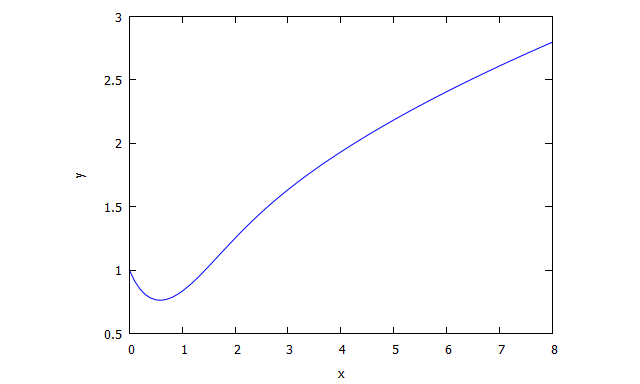
\includegraphics[width=0.75\textwidth]{DE_rk1.png}
	\caption{Plot of the return value of function rk having solved one first-order ODE with the Runge-Kutta method.}
	\label{DE-Fig1}
\end{SCfigure}

\lz \begin{small}
\color{blue}
\begin{lstlisting}
<@\tcr{(\%i1)}@   res: rk([4-y1^2-4*y2^2,y2^2-y1^2+1],[y1,y2],[-1.25,0.75],[x,0,4,0.02])$
<@\tcr{(\%i2)}@   plot2d ([[discrete, makelist([p[1],p[2]],p,res)],[discrete, makelist([p[1],p[3]],p,res)]],[legend,"y_1","y_2"])$
\end{lstlisting}
\color{black}
\end{small}

\lz Figure \ref{DE-Fig2} shows the resulting plot.

\begin{SCfigure}[0.33][h]
	\centering
	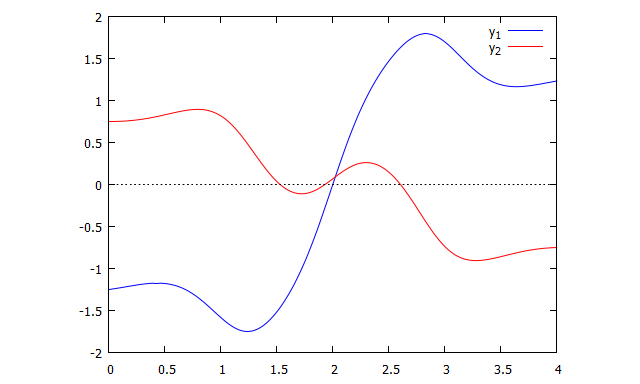
\includegraphics[width=0.75\textwidth]{DE_rk2.png}
	\caption{Plot of the return value of function rk having solved a system of two first-order ODEs with the Runge-Kutta method.}
	\label{DE-Fig2}
\end{SCfigure}

\section{Graphical estimate}

\subsection{Direction field}

Direction fields can be plotted either with function \emph{plotdf}, which uses xMaxima, or with function \emph{drawdf}, which uses Gnuplot's \emph{draw}.

\subsubsection{plotdf}

\emph{plotdf} is a function to plot the direction field of one or two first-order ODEs, possibly together with the specific solution of an initial value problem (IVP). \emph{plotdf} uses xMaxima and depends on it being installed; but it can be used also from other interfaces, e.g. wxMaxima or the console. \emph{plotdf} can export plots only in postscript format (.ps). External programs can be used to transform such files into .jpg or .png format; we use the downloadable freeware \emph{XnConvert}. \index{XnConvert}

\lzz \hyt{plotdf}{\tcr{\emph{plotdf ($ \gpal eq \gbar [eq_1,eq_2] \gpar \, \glangle, [x,y] \grangle \glangle, [opt_1], \dots, [opt_n] \grangle $)}}} \hfill \tcr{[function]}\index{plotdf}

\lz Creates a plot of the direction field of either one first-order ODE or a system of two of them, given in explicit form. In the first case, \emph{eq} is the right-hand side of the ODE
\begin{equation*}
	y'(x) = F(x,y),
\end{equation*}
while in the second case, the list $ [eq_1,eq_2] $ contains the right-hand sides of the ODEs
\begin{equation*}
	x'(t) = F_1(t,x) \teee{and} y'(t) = F_1(t,y).
\end{equation*}
In the first case, the second argument provides the names of the independent and the dependent variable; in the second case, it provides the two dependent variables, the independent variable always being \emph{t}. The second argument can be omitted in either case, if the names are \emph{"x"} and \emph{"y"}.

\lz The following options, each of them enclosed in a list and separated by commas, can be used:

\lz \tcr{[trajectory\_at,$ x_0,y_0 $]}: Initial value problem (IVP) with initial values $ x_0, y_0 $.

\lz As a first example, we plot the direction field of the first-order ODE
\begin{equation*}
	y'(x)= e^{-x} y
\end{equation*}
together with an IVP given by $ x_0=2, \, y_0=y(x_0)=-0.1 $.

\lz \begin{small}
\color{blue}
\begin{lstlisting}
<@\tcr{(\%i1)}@   rk(t-x^2,x,1,[t,0,8,0.1])$
<@\tcr{(\%i2)}@   plot2d ([discrete, %])$
\end{lstlisting}
\color{black}
\end{small}

\lz Figure \ref{DE-Fig3} shows the resulting plot. 

\begin{SCfigure}[1.0][h]
	\centering
	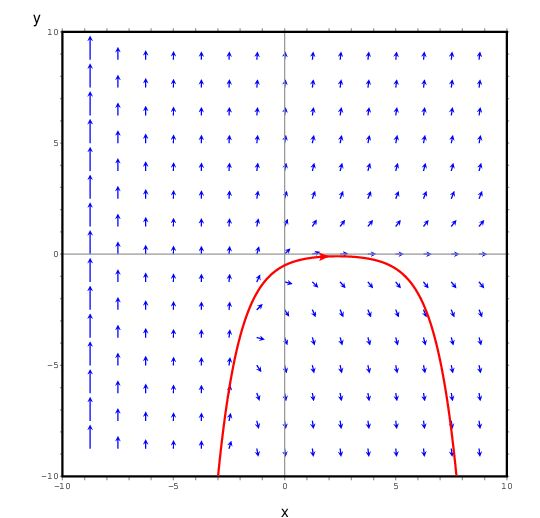
\includegraphics[width=0.5\textwidth]{DE_plotdf1.jpg}
	\caption{Plot of the direction field of a first-order ODE together with an IVP.}
	\label{DE-Fig3}
\end{SCfigure}

\subsubsection{drawdf}

\end{document}